\documentclass[a4paper, 10pt]{article}

\usepackage{wrapfig}
\usepackage{listings}
%Math
\usepackage{amsmath}
\usepackage{amsfonts}
\usepackage{amssymb}
\usepackage{amsthm}
\usepackage{ulem}
\usepackage{textcomp}


%PageStyle
\usepackage[german]{babel}
\usepackage{fontenc}
\usepackage{fancyhdr, graphicx}
\usepackage{fullpage}
\usepackage{graphicx}
\usepackage{textcomp}
\usepackage{fancyhdr} %for header/footer
\usepackage{wrapfig}


\newcommand{\Bold}[1]{\textbf{#1}} %Boldface
\newcommand{\Kursiv}[1]{\textit{#1}} %Italic

%Metadata
\title{Betriebssysteme}
\author{Fabian Stebler \& Jan F\"assler}
\date{2. Semester (FS 2012)}


\begin{document}
\maketitle
\newpage
\section{Einleitung}

\subsection{Anforderungen an ein Betriebssystem}
\begin{itemize}
	\item Start des Systems
	\item Laden und Unterbrechen von Programmen
	\item Methoden für die Interprozesskommunikation
	\item Verwaltung der Prozessorzeit
	\item Verwaltung des primären und sekundären Speicherplatzes für das Betriebssystem und seine Anwendungen
	\item Verwaltung der angeschlossenen Geräte, Netzwerke etc.
	\item Schutz des Systemkerns und seiner Ressourcen vor nicht intendierter Benutzung
	\item Benutzerführung, Rollen \& Rechte	
	\item Einheitliche Schnittstelle für die System- \& Anwendungs- programmierung
	\item Ereignisprotokollierung
\end{itemize}
\subsection{Definition}
Ein Betriebssystem ist die Software die die Verwendung eines Computers erm\"oglicht. Es verwaltet Betriebsmittel wie den Speicher, die I/O-Ger\"ate, usw.
\subsection{Bestandteile}
Betriebssysteme bestehen in der Regel aus einem Betriebssystemkern (englisch: Kernel), der die Hardware des Computers verwaltet, sowie grundlegenden Programmen, die dem Start des Betriebssystems und dessen Konfiguration dienen.\\
Zu den Komponenten z\"ahlen:
\begin{itemize}
\item Boot-Loader
\item Ger\"atetreiber
\item Systemdienste
\item Programmbibliotheken
\item Dienstprogramme
\item Anwendungen
\end{itemize}

\subsection{Varianten von Betriebssystemen}
\begin{itemize}
\item Einbenutzer- und Mehrbenutzersysteme
\item Einzelprogramm- und Mehrprogrammsysteme
\item Stapelverarbeitungs- und Dialogsysteme
\end{itemize}
Betriebssysteme finden sich in fast allen Computern: als Echtzeitbetriebssysteme auf Prozessrechnern, auf normalen PCs und als Mehrprozessorsysteme auf Hosts und Grossrechnern.

\subsection{Geschichte}
Mechanische Rechenmaschienen wurden mit der Zeit mit Lochstreifen versehen und somit konnte von einer Art Betriebssystem gesprochen werden. Sp\"ater wurden die mechanischen Teile durch die R\"ohrentechnologie und anschliessend durch Transistoren ersetzt (ca.1947).
\begin{itemize}
\item 1955 Erfindung Mikroprogrammierung
\item 1964 Erstes modellreihen\"ubergreifendes BS
\item 1969 Beginn Arbeit an UNIX
\item 1972-1974 Umschreiben UNIX in C (portabilit\"at)
\item 1980-1990 Popularit\"atssteigerung bei Heimcomputern
\item 1981 Entwicklung erste graphische Oberfl\"ache. Apple kauft sich mit Aktien ein, kreirt MAC und MAC OS. Verliert aber aufgrund der Experimentierfreudigkeit Marktanteile an Windows.
\item 1991 Linus Torvalds beginnt mit der Entwicklung des LINUX-Kernels. (Start Open Source Bewegung)
\item Microsoft entwickelte MS-DOS weiter und liefert MS-Windows
95 Mitte der 90‘er Jahre aus. (Tabellenkalkulation)
\item Im PC-Desktop-Bereich tobte ein eigentlicher „Glaubenskrieg“ zwischen Microsoft und Apple.
\item IBM und andere zogen sicher immer mehr in den Midrange/Mainframe-Markt zur\"uck.
\end{itemize}

\subsection{Lessons learned}
\begin{itemize}


\item Die Grundkonzepte haben sich stark angen\"ahert.
\item Kompatibilit\"at wird (oft z\"ahneknirschend) bereitgestellt.
\item Entscheide f\"ur/gegen ein Betriebssystem (bes. im Privat-
bereich) haben teilweise weltanschauliche Hintergr\"unde.
\item Der Quellcode ist kein Geheimnis und kein Marktvorteil mehr.
\item Partizipative Entwicklung durch Communities hat ein grosses
Markt- und Sparpotential.
\item Die Positionen scheinen bezogen, der Markt w\"achst immer
noch stark genug, um den etablierten Anbietern Wachstum zu
erm\"oglichen.
\item Die Wertsch\"opfung hat sich verlagert:
\begin{itemize}
\item Hardware zu Betriebssystem
\item GUI zu Applikationen
\item Daten zu Business Intelligence
\end{itemize}
\end{itemize}
\newpage

\section{Blockstruktur eines Betriebssystems}
\subsection{Aufgaben des Betriebssystems}
\begin{itemize}
\item Start des Systems
\item Laden und Unterbrechen von Programmen (Laufzeitumgebung)
\item Methoden f\"ur die Interprozesskommunikation
\item Verwaltung der Prozessorzeit
\item Verwaltung des prim\"aren und sekund\"aren Speicherplatzes f\"ur das Betriebssystem und seine Anwendungen
\item Verwaltung der angeschlossenen Ger\"ate, Netzwerke etc.
\item Schutz des Systemkerns und seiner Ressourcen vor nicht intendierter Benutzung
\item Benutzerf\"uhrung, Rollen und Rechte
\item Einheitliche Schnittstelle f\"ur die System- und Anwendungsprogrammierung Ereignisprotokollierung

\end{itemize}

\subsection{Grapische Darstellung}
Untenstehende Grafik zeigt die Schichtenarchitektur eines modernen Betriebssystems (Linux).\\
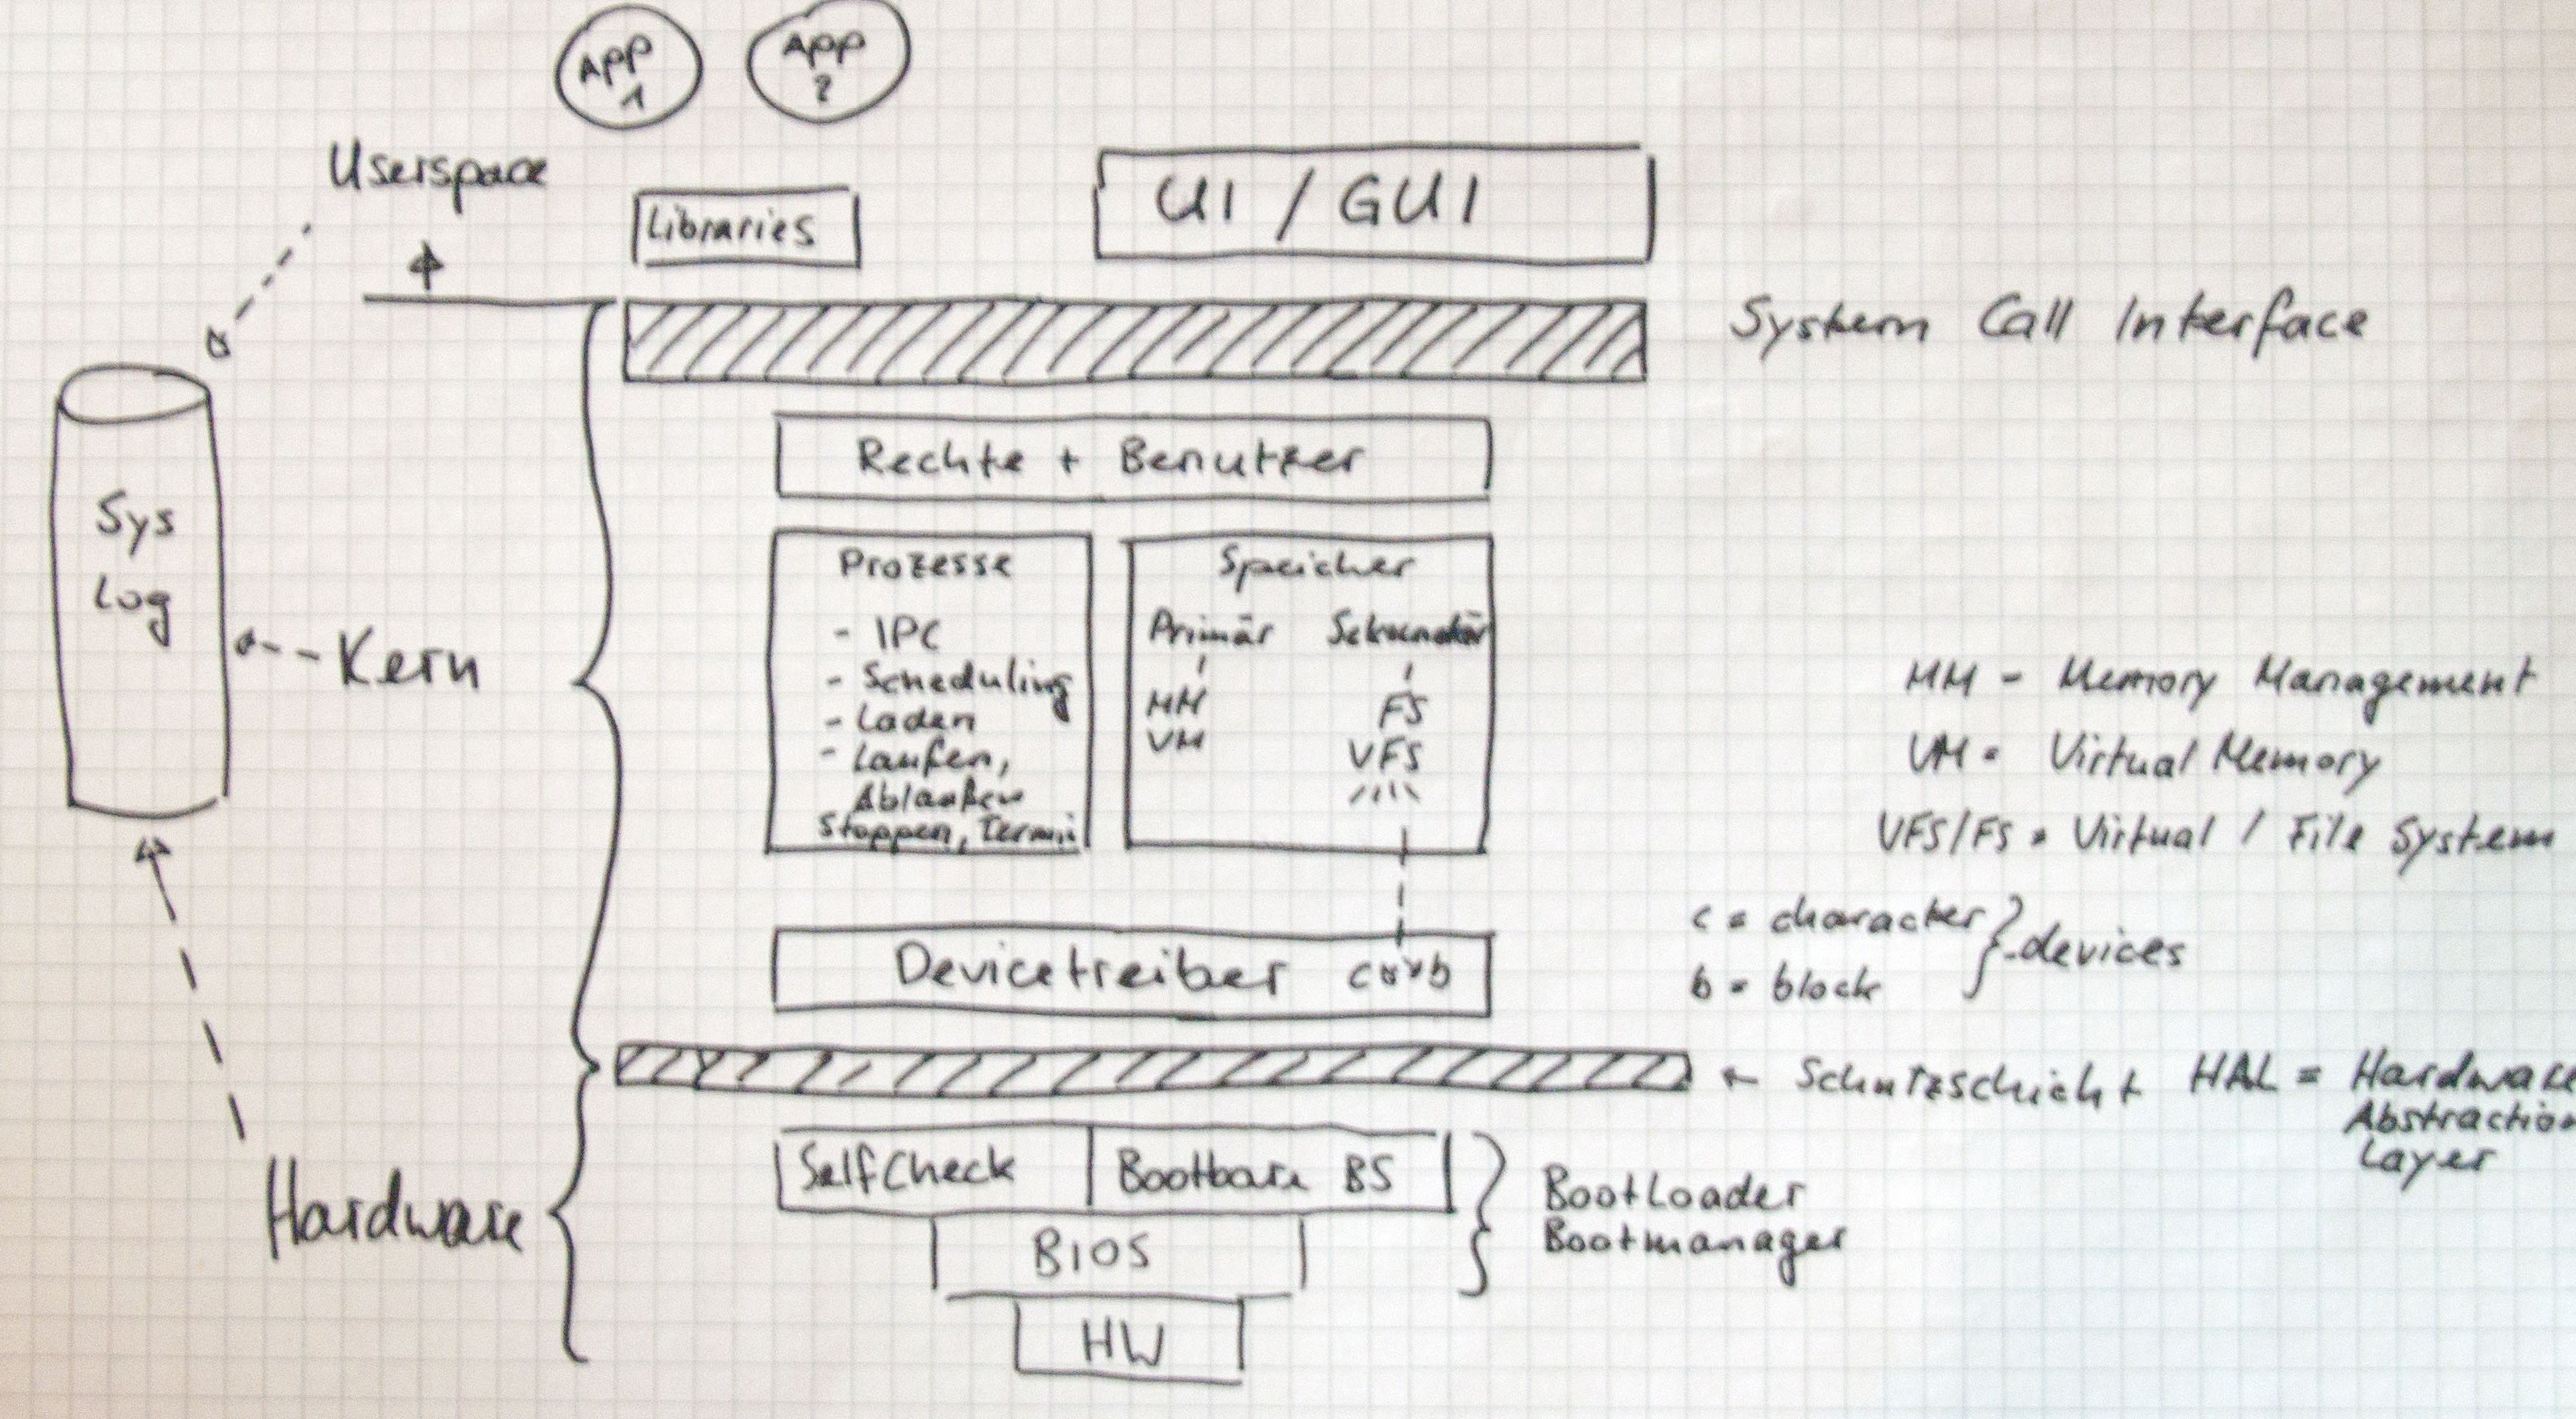
\includegraphics[scale=0.15]{Bsys.jpg}\\

\subsection{Aufgabenteilung der Bl\"ocke}
\subsubsection{Dateisystem}
\begin{itemize}
\item Struktur des Dateisystems (Baum, Graph, flach, ...)
\item Strukturelemente (Directories)
\item Zugriffsrechte auf Directories und Dateien
\item Anlage, Suche, Manipulation, L\"oschen von Dateien
\item Verwaltung von Datenbl\"ocken auf Speichermedien
\item Kombination von Dateisystemen (mounting)
\item Benutzerschnittstelle und Navigation
\item Backup / Restore
\end{itemize}

\subsubsection{Prozesssteuersystem}
\begin{itemize}
\item Prozesse kreieren
\item Prozesse starten
\item Prozesse schedulen, Warteschlangen, Ressourcenverbrauch
\item Prozesse stoppen / unterbrechen
\item Prozesse terminieren (freiwillig / wegen Fehler)
\item Prozesskommunikation (Prozess-Prozess und Kern-Prozess / Prozess-Kern)
\item Zuordnung von Hauptspeicher und anderen geteilten Ressourcen
\item Ein-/Auslagerung von Prozessen
\item Prozesse und ihre Zust\"ande anzeigen
\end{itemize}

\subsubsection{System Call Interface}
\begin{itemize}
\item Einzige Schnittstelle zwischen Kern und Benutzer
\item Normierung der Syntax und Semantik (POSIX 1003)
\item Parametrisierung und \"ubergabe
\item \"ubergabe der Kontrolle $\rightarrowtail$ Betriebsmodi
\end{itemize}

\subsubsection{Programmierung}
\begin{itemize}
\item Wahl der Programmiersprache / Systempr\"aferenz
\item System-/Applikationsnahe Bibliotheksfunktionen
\item Programmierumgebung (Editor, Compiler, Assembler, Linker, Loader, Debugger)
\item „Bundling“ in einer Applikation (z.B. Eclipse)
\end{itemize}

\subsubsection{Benutzerschnittstelle}
\begin{itemize}
\item Textuelle Basis-Schnittstelle mit Kommando-Interpreter (Shell) Konsole
\item Programmierbarkeit (Scripting, Pipelining, I/O-Redirection) der Benutzerschnittstelle
\item Graphische Benutzerschnittstelle (GUI) mit
\item Abstraktion der unterliegenden Komplexit\"at und Syntax f\"ur Nicht Systemspezialisten
\item Austauschbarkeit der Shell und der Systembefehle (Applikationen)
\end{itemize}


\subsubsection{I/O Management}
Ein Betriebssystem muss auch die Hardware kontrollieren:
\begin{itemize}
\item Die F\"ahigkeiten der Hardware voll aussch\"opfen.
\item Die verschiedenen inhomogenen Komponenten zu einer Einheit formen.
\item Die Hardware sch\"utzen vor unerlaubtem Zugriff.
\end{itemize}
Anm.: Peripherieger\"ate sind meist unterschiedlich, sollten aber leicht in das System integrierbar sein.

\subsubsection{File System als generelle Schnittstelle}
Die Idee von Unix war, dass File System f\"ur m\"oglichst viele Subsysteme als Schnittstelle zu verwenden.
\begin{itemize}
\item Dateien, Directories
\item Prozesssynchronisation (Lock Files, ...)
\item Prozesskommunikation (Pipes, Sockets)
\item Peripherieger\"ate (Device Special Files)
\item Kommunikationsprotokolle (TCP/IP, ...)
\item Prozesse (/proc Dateisystem)
\end{itemize}
Anm.: Es bedingt einer zus\"atzlichen Abstraktionsschicht.

\newpage
\section{Filesystem}
Die anschliessende Graphik zeigt ein virtuelles Dateisytem:\\
\\
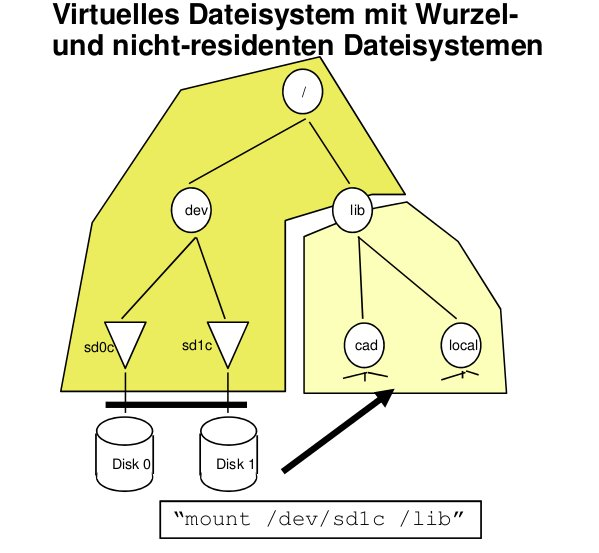
\includegraphics[scale=0.4]{Dateisystem.jpg}\\

\subsection{Partition auf der Disk}
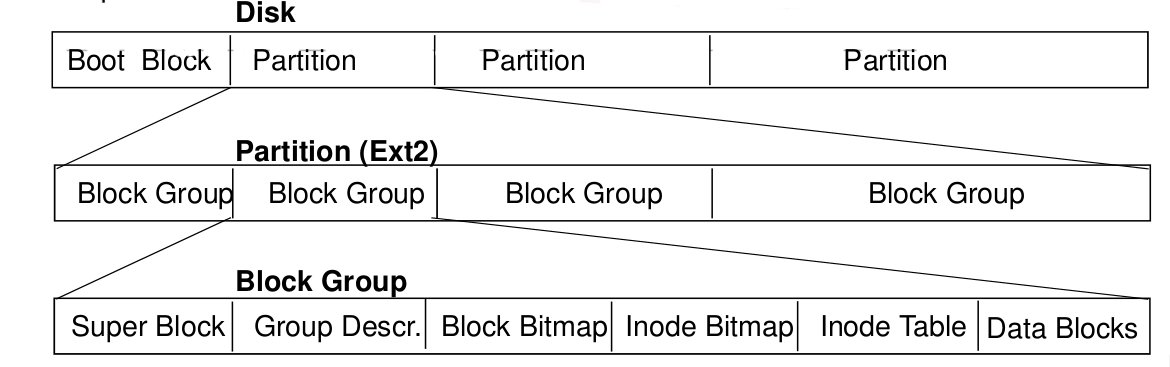
\includegraphics[scale=0.3]{Partition_HD.jpg}\\
\\
Superblockinhalt:
\begin{itemize}
\item Anzahl inodes und Datenbl\"ocke
\item Adresse des 1. Datenblocks
\item Anzahl freie Bl\"ocke und inodes
\item Gr\"osse eines Datenblocks
\item Bl\"ocke / inodes pro Gruppe
\item Anzahl Bytes pro inode
\end{itemize}

\subsection{Blockallokationen}
\subsubsection{Zusammenh\"angende Belegung}
Vorteile:
\begin{itemize}
\item Einfachste aller Methoden
\item Sehr schneller direkter Zugriff auf die Daten
\item F\"ur die Lokalisierung der Dateibl\"ocke brauchen wir
nur Anfangsblock und Gr\"oße der Datei zu wissen.
\item Lese-Operationen k\"onnen sehr effizient implementiert
werden.
\item Gute Fehlereingrenzung
\end{itemize}
Nachteile:
\begin{itemize}
\item Dynamische Dateigr\"oßen sind ein Problem
\item Im Laufe der Zeit wird die Platte fragmentiert.
\item Platz zu finden f\"ur neue Dateien ist ein Problem
\item Verwaltung von freien Speicherpl\"atzen notwendig
\item Regelm\"aßige Kompaktifizierung notwendig
\item Platte hin- und zur\"uck kopieren
\end{itemize}
\subsubsection{Verlinkte Bl\"ocke}
Jede Datei wird als verkettete Liste von Plattenbl\"ocken gespeichert. Nur die Plattenadresse des ersten und letzten Blocks wird in dem Verzeichniseintrag gespeichert.\\
Vorteile:
\begin{itemize}
\item Keine externe Fragmentierung
\item Sequenzieller Zugriff ist kein Problem
\end{itemize}
Nachteile:
\begin{itemize}
\item Schlechter wahlfreier Zugriff auf Dateiinhalte
\item Jeder Verweis verursacht einen neuen Plattenzugriff
\item Overhead f\"ur das Speichern der Verkettung (L\"osung: clusters aus mehren Bl\"ocken)
\item Erh\"ohter Aufwand bei Dateizugriffen
\item Schlechte Fehlereingrenzung
\end{itemize}

\subsubsection{Filemap (Landkarte)}
\begin{wrapfigure}{r}{8cm}
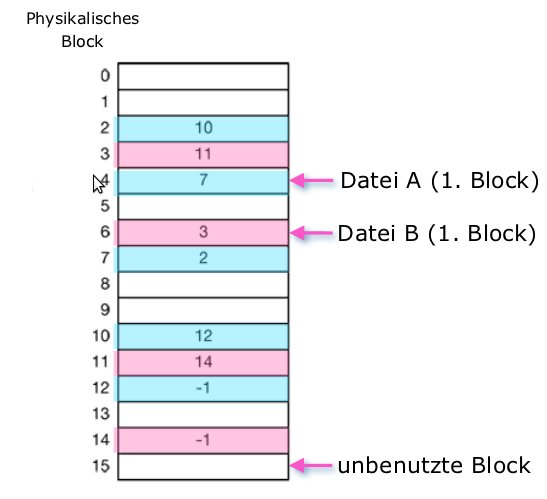
\includegraphics[scale=0.4]{filemap.jpg}
\end{wrapfigure}

Vorteile:
\begin{itemize}
\item Dateien k\"onnen sehr leicht und effizient vergr\"oßert werden
\end{itemize}
Nachteile:
\begin{itemize}
\item Interne Fragmentierung
\item schlecht f\"ur random accesses
\item fehleranf\"allig
\end{itemize}
\newpage
\subsubsection{Index Allokation}
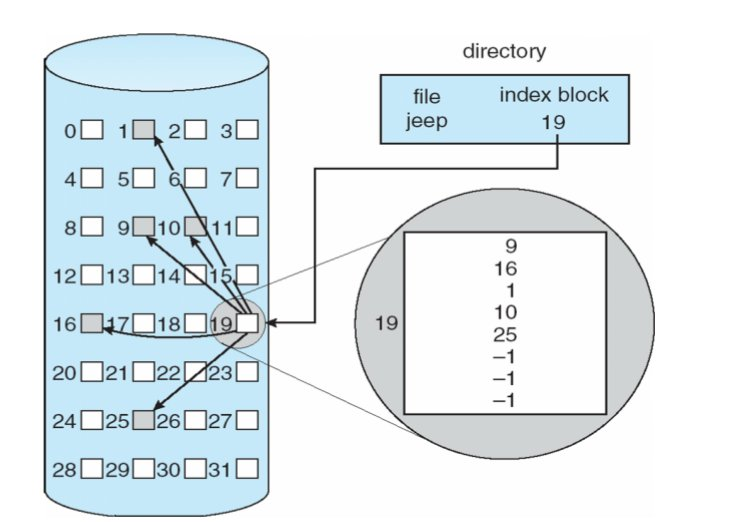
\includegraphics[scale=0.5]{index_allocation.jpg}

\subsection{Struktur von Inodes}
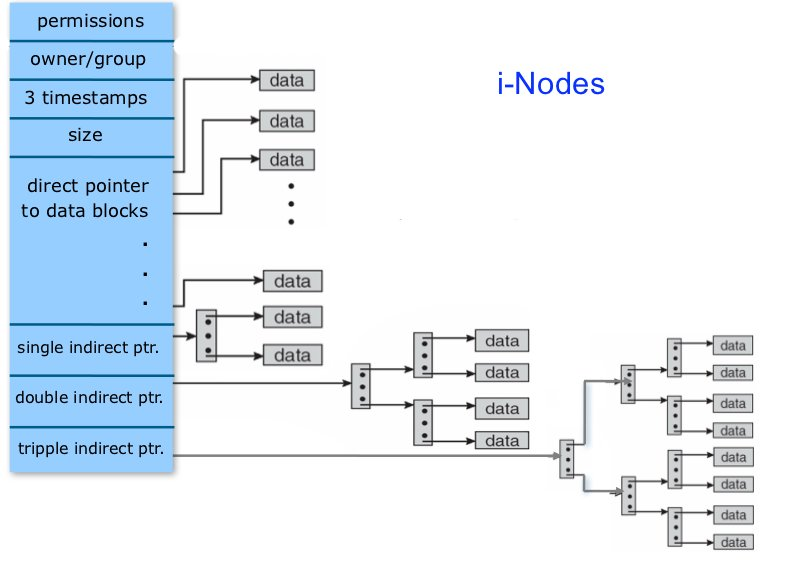
\includegraphics[scale=0.6]{inodes.jpg}

\subsubsection{Informatione Inode}
\begin{tabular}{p{7cm}|p{7cm}}
\textbf{Auf der Disk} & \textbf{Zus\"atzlich im Memory} \\ \hline
\begin{itemize}
\item Inode Nummer
\item Anzahl hard links
\item Typ (-, l, d, b, c, p)
\item Rechte (-, r, w, x, s)
\item Besitzer
\item Gruppe
\item Gr\"osse
\item Letzte “access time”
\item Letzte “content change time”
\item Letzte “inode modification time”
\item Datenblock Information
\end{itemize}
&
\begin{itemize}
\item Link auf die “hash list”
\item Link auf die “inode list”
\item Benutzerz\"ahler
\item Ger\"atenummer
\item “Device special file” Indikator
\item Gr\"osse eines Blocks
\item Anzahl Bl\"ocke
\item Lock auf den inode
\item “Mount point” Indikator
\item Warteschlange wartender Prozesse
\item Locks auf die Datei
\item Hauptspeicher-Region (f\"ur Memory-mapped file I/O)
\item Belegte Seiten im Hauptspeicher
\end{itemize}
\end{tabular}

\subsection{Designvorgaben f\"ur Filesystem}
\begin{itemize}
\item Anzahl Disks und Disk Controller
\item Verteilung auf Partitionen
\item Blockgr\"osse pro Partition
\begin{itemize}
\item Grosse Bl\"ocke: schneller Zugriff auf Dateien (Datei-Durchschnittsgr\"osse $<$ 4 kB)
\item Kleine Bl\"ocke: weniger interne Fragmentierung
\end{itemize}
\item Anzahl Dateien / Inodes pro Partition
\begin{itemize}
\item Wenige Inodes: mehr Platz f\"ur Dateibl\"ocke
\item Viele Inodes: mehr Dateien pro Partition mgl.
\end{itemize}
\end{itemize}

\newpage
\section{Prozesse}

\subsection{Einleitung}

\subsubsection{Was ist ein Prozess?}
Ein oder mehrere Programme (deterministische Sequenz von Instruktionen) werden auf einem oder mehreren physischen oder virtuellen Prozessoren ausgeführt. Zu jedem Zeitpunkt der Ausführung verbunden mit einem “computational state” (aktuell verwendete Variablen etc. im Programm), externe Ressourcen wie Zustand der CPU, Register, Zeitnahme, usw. Ein Prozess wird durch das Betriebssystem strikt überwacht und verwaltet

\subsubsection{Anforderungen an ein Prozess-Steuersystem}
\begin{itemize}
	\item Prozesse kreieren
	\item Prozesse starten
	\item Prozesse schedulen, Warteschlangen, Ressourcenverbrauch
	\item Prozesse stoppen / unterbrechen
	\item Prozesse terminieren (freiwillig / wegen Fehler)
	\item Prozess-Signalisierung und -kommunikation
	\item Faire Zuordnung von Hauptspeicher und anderen geteilten Ressourcen
	\item Ein-/Auslagerung von Prozessen bei vollem Speicher
	\item Prozesse und ihre Zustände anzeigen
\end{itemize}

\subsubsection{Unix-Prozess Segmente}
\begin{itemize}
	\item Text Segment (8 K)
	\item Daten Segment (32 K)
	\item Stack Segment (64 K)
	\item Shared Memory Segment
	\item Mapped File Segment
\end{itemize}

\subsection{Kernel und User Mode}
Ein Prozess hat mindestens (in Unix genau) zwei Ausführungsmodi:
\begin{description}
	\item[User Mode:] Es wird der normale Programmcode ausgeführt.
	\item[Kernel Mode:] Ss werden Systemaufrufe ausgeführt oder Ausnahmen behandelt.
\end{description}
Der Übergang erfolgt durch einen Systemaufruf durch das Programm, eine Ausnahmesituation (Fehler) oder durch asynchrone Events (Kom- munikation etc). Beide Modi haben separate Segmente und sind voneinander abgeschirmt.

\subsubsection{Prozess-/Kontext- Wechsel}
Wenn ein Prozess:
\begin{itemize}
	\item warten muss (z.B. auf I/O oder einen Event),
	\item seine zugeordnete Laufzeit oder andere Ressourcen- grenzen erreicht bzw. überschreitet,
	\item terminiert oder gestoppt wird,
	\item die CPU freiwillig abgibt
\end{itemize}
muss das Betriebssystem die CPU einen anderen ablaufbereiten Prozess zuteilen und diesen starten. Dies erfordert das Abspeichern des exakten Prozess- Zustandes und das spätere Restaurieren, wenn der Prozess wieder weiterlaufen soll.\\

\begin{wrapfigure}{r}{7cm}
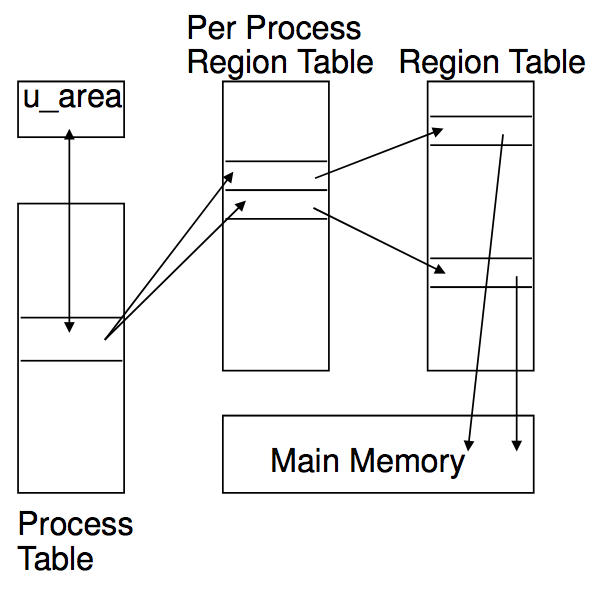
\includegraphics[scale=0.2]{process_region_table.png}
\end{wrapfigure}

\subsubsection{Kernel-Datenstrukturen für das Prozess-Management}
In älteren Unix-Varianten ist die Grösse der Prozesstabelle statisch (schnelle Indexierung, Lizenzierung über Anzahl Prozesse / Benutzer).\\
Alternativ kann die Prozesstabelle eine verkettete Liste sein (variable Anzahl Prozesse, aber komplizierte Indexierung und Überlauf-Gefahr). \\
Linux verwendet eine Mischform (dynamisch angelegte Prozesskon- trollblöcke (PCB) in einer verketteten Liste mit einer statischen Hash- Tabelle für die schnelle Suche).

\subsection{Sichern des Prozess Kontexts}
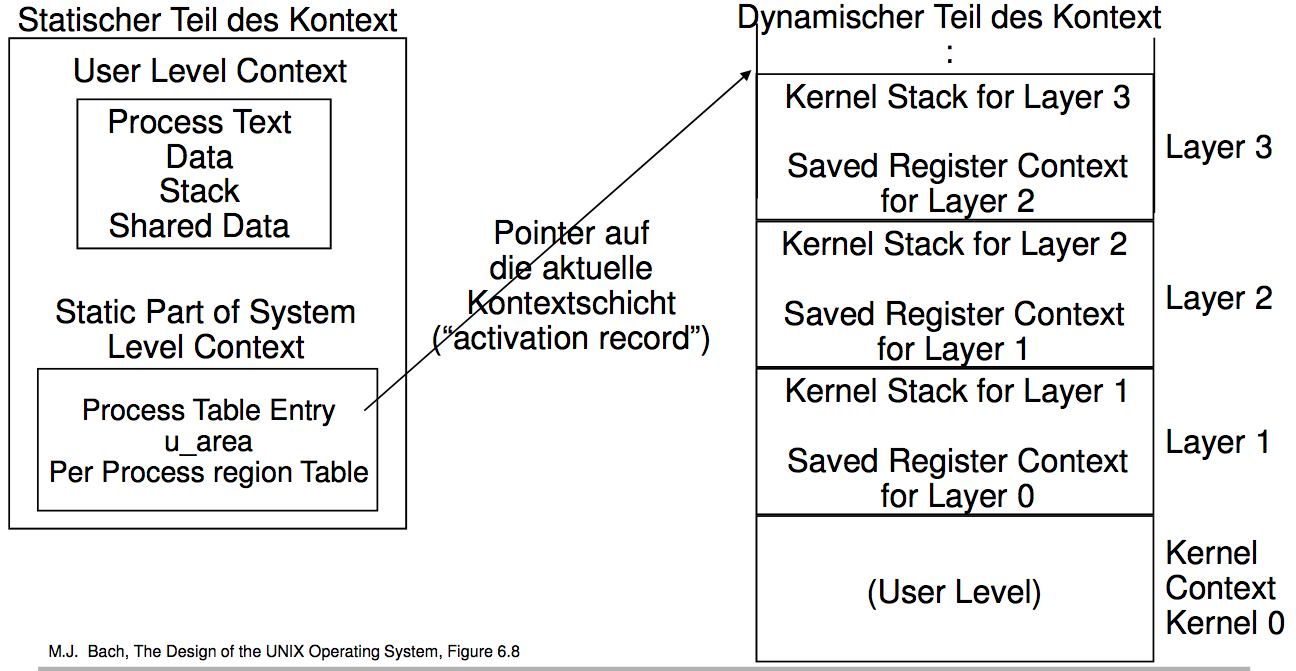
\includegraphics[scale=0.3]{save_process_context.png}

\subsection{Prozess Zust\"ande}
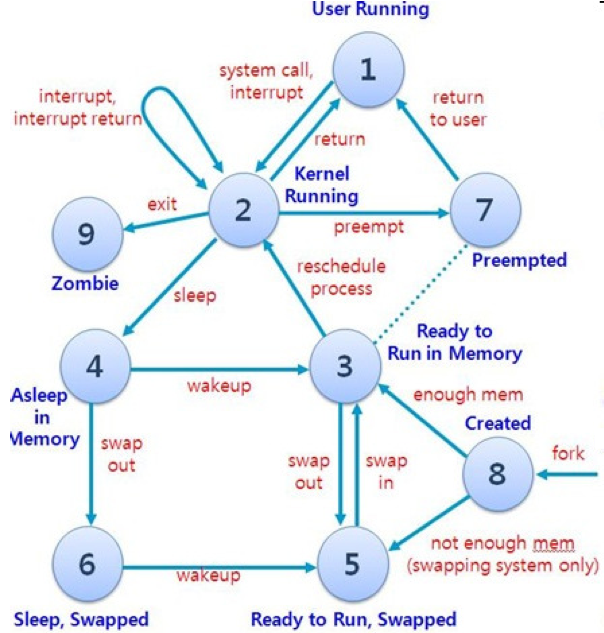
\includegraphics[scale=0.5]{process_states.png}

\subsection{Prozess-bezogene System Calls}
\begin{description}
	\item[fork] Erstellen eines neuen Prozesses durch Kopieren
	\item[exec] AusführeneinesneuenProgrammsineiner vorhandenen Prozesshülle
	\item[Signal] Stoppen eines Prozesses
	\item[exit] Terminieren eines Prozesses
	\item[wait] Warten auf das Terminieren eines Prozesses, einfache Synchronisation
\end{description}

\subsection{Prozesse versus Threads}
Kontextwechsel sind eine “schwere” Operation mit viel Verarbeitungsaufwand durch den Kernel. Da viele Unix-Prozesse I/O-intensiv sind, verbringen sie die meiste Laufzeit mit Warten, dadurch erhöht sich die Anzahl von Kontextwechseln im System. Neuere Unix-/Linux-Systeme unterstützen mehr als einen parallelen Ausführungspfad innerhalb eines Prozesses (multi-threading). Es muss kein Kontextwechsel vorgenommen werden, um eine andere Aktivität zu starten. \\
Aber:
\begin{itemize}
	\item Das Scheduling muss innerhalb des Prozesses erfolgen,
	\item die Threads sind verwandt, d.h. ihr Code liegt innerhalb des gleichen Unix-Prozesses,
	\item der Programmierer muss für die Datenintegrität selbst sorgen.
\end{itemize}
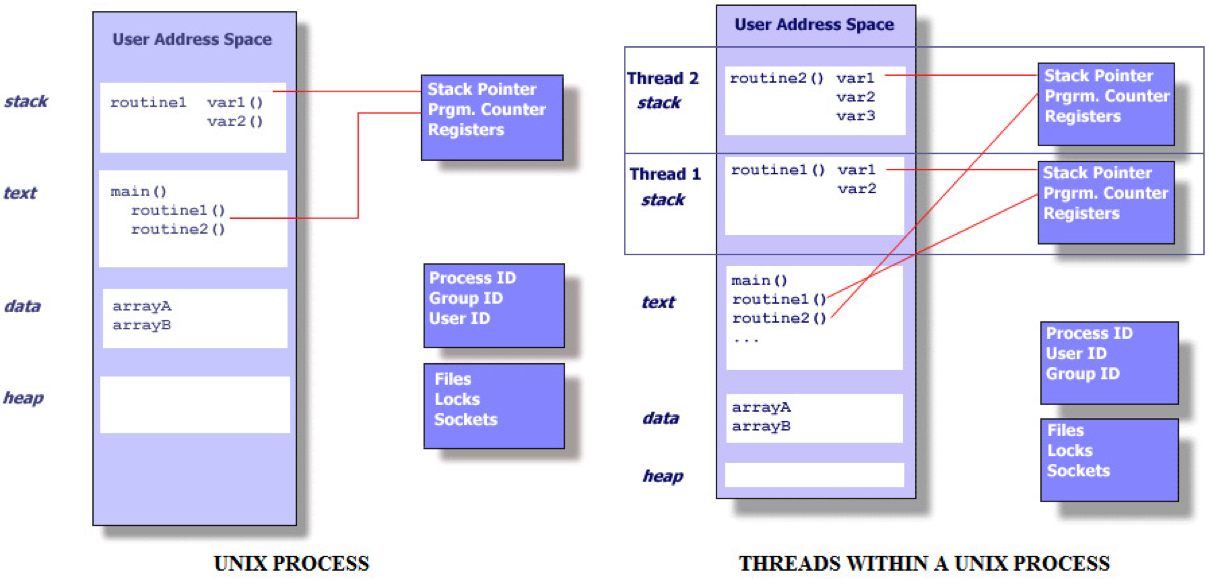
\includegraphics[scale=0.3]{process_vs_threads.png}

\subsubsection{Basismodell für Threads}
\begin{itemize}
	\item Kernel-Code (System Call Interface) oder Library?
	\item Ausführungsmodelle
		\begin{itemize}
			\item Master/Slave(s)
			\item Cooperating Pool
			\item Pipeline
			\item Hybrid
		\end{itemize}
	\item Besondere Anforderungen
		\begin{itemize}
			\item Synchronisation
			\item Betriebsmittel-Zuteilung (Scheduling)
			\item Ausnahmebehandlung
		\end{itemize}
\end{itemize}

\subsubsection{Benutzungs- und Administrationssicht auf ein Prozess-Steuersystem}
\begin{itemize}
	\item Prozess-Erzeugung und –Termination
	\item Identifikation
	\item Priorisierung
	\item Besitzer	
	\item Ressourcenverbrauch
	\item Prozess-Ein-/Auslagerung
	\item Signalisierung
	\item Prozesskommunikation
\end{itemize}

\newpage
\section{Hauptspeicherverwaltung}
\subsection{Virtual Memory}
\begin{itemize}
\item Hauptspeichererweiterung pro einzelnes System oder Prozess.
\item Systematische Abstraktion f\"ur systemspezifische Overlay-
Techniken
\item Organisation des Hauptspeichers in gleich grosse,
einheitlich adressierbare Einheiten (Seiten, pages)
\item Ben\"otigt hardware-unterst\"utze Abbildung zwischen
physischen und virtuellen Adressen
\end{itemize}

\subsection{Swapping}
Swapper (Process 0) wird periodisch vom Kernel aufgerufen.\\

Swap Device  $\longleftrightarrow$ Swapper $\longleftrightarrow$ Hauptspeicher\\

Swap Out (Hauptspeicher zu SwapDevice):
\begin{itemize}
\item Kein Platz im HS f\"ur weitere Prozesse, Prozess ruft aber fork auf $\Rightarrow$ fork swap
\item Kein Platz im HS aber Prozess w\"achst, weil z.B. Stack w\"achst $\Rightarrow$ expansion swap
\item Swap Device ausgelagerter wartender Prozess wird ready to run und wird vom Scheduler ausgef\"uhrt $\Rightarrow$ exchange swap
\end{itemize}

Swap In (SwapDevice zu Hauptspeicher):
\begin{itemize}
\item Nur ready to run Prozesse sind w\"ahlbar $\Rightarrow$
\item Pr\"aferenz auf Prozesse die > 2 sec. Ausgelagert waren
\end{itemize}

\subsection{Demand Paging}
Anforderung: ein einzelner Prozess soll gr\"osser sein d\"urfen, als der
verf\"ugbare Hauptspeicher.\\
\\
Voraussetzungen:
\begin{itemize}
\item Hardware unterst\"utzt seitenorientieres Speichermanagement (1$/$2 $–$ 4 kB / Seite)
\item Wiederaufsetzbare CPU-Instruktionen (wenn Instruktionen \"uber eine Seiten-
grenze verlaufen)
\end{itemize}

Idee:\\
Nur die gerade verwendeten Teile des Codes werden geladen. Dies sind 10 bis 15 
Prozent die im HS liegen (working set). Wird auf eine Seite zugegriffen die nicht geladen ist, so gibt es einen page fault und die Seite wird nachgeladen.\\

Optimierung des “demand paging” durch
\begin{itemize}
\item Reference bit $\rightarrow$ erm\"oglicht nicht-lineares “working set”
\item Age bit $\rightarrow$ verbleibende Zet einer Seite im “working set”
\end{itemize}
Zwei Aufgaben f\"ur das Paging-Subsystem:
\begin{itemize}
\item Seitenalterung und Auslagerung/L\"oschung gen\"ugend alter Seiten
\item Bearbeitung von “page faults”
\end{itemize}

\newpage
\section{I/O, Peripherie}
\subsection{Anforderungen von Peripheriegeräten}
\begin{itemize}
	\item Ressourcenverwaltung:
		\begin{itemize}
			\item Hauptspeicher für Zwischenpufferung von Daten beim Transfer
			\item CPU-Zeit für das Behandeln asynchroner Events (z.B. Ankunft von Daten an der Netzwerkschnittstelle)
		\end{itemize}
	\item Zugriffssteuerung und –synchronisation:
		\begin{itemize}
			\item Einheitliche Schnittstelle
			\item Synchronisation von Zugriffen durch die Prozesse
			\item Signalisierung
		\end{itemize}
	\item Scheduling
\end{itemize}

\subsection{Aufgaben und Funktionsweise des I/O-Subsystems}
\begin{itemize}
	\item Aufgabe: schneller und zuverlässiger Datentransfer zwischen Geräten (Disk, Drucker, Tastatur, Bildschirm, Maus etc.) und Prozessen, d.h. Datenstrukturen im Prozess-Adressraum (read und write Operationen)
	\item Design: Das I/O Subsystem besteht aus einer oberen Schicht, die Daten zwischen dem Benutzer- und dem Kernel-Adressraum bewegt, und einer unteren Schicht, die Daten zwischen dem Kernel-Adressraum und den Geräten bewegt.
	\item Standardisiertes I/O (Geräteunabhängigkeit bezüglich Programmierung und Benutzung)
	\item Optimiertes I/O (abhängig vom Gerät und dessen Eigenschaften, Durch- satz, Sicherheit usw.)
	\item Konsistenz trotz Unterbrechbarkeit der Operationen und Zugriffssicher- heit wenn Daten zwichen Kernel und Benutzer-Prozess bewegt werden
	\item Drei Typen von I/O: Datei-basiert, Zeichen-basiert, STREAM-basiert
\end{itemize}

\subsection{Buffer-Cache}
\subsubsection{Der klassische Buffer Cache}
\begin{itemize}
	\item Ziel: Optimierung des Zugriffs auf block-orientierte geräte, maximale Menge Daten im Speicher behalten.
	\item Strategie 1: vorausschauendes Lesen (read ahead)
		\begin{itemize}
			\item Vorteil: beschleunigt das sequentielle Lesen (z.B. einer Datei)
			\item Risiko: potentielle Verschwendung von Hauptspeicher
		\end{itemize}
	\item Strategie 2: verzögertes Schreiben (delayed write)
		\begin{itemize}
			\item Vorteil: Bündeln von Daten in Blöcke für das Schreiben auf langsame Geräte (z.B. Disk)
			\item Risiko:nacheinemerfolgreichenwrite()Systemaufrufsind die Daten noch nicht auf der Disk gespeichert (Verlustrisiko)
		\end{itemize}
	\item Optimiert für die Arbeit mit dummen Peripheriegeräten
\end{itemize}
\subsubsection{Der neue Buffer Cache}
Der neue Buffer Cache verwendet einen seitenorientierten Zugriff auf Dateien, ähnlich der Hauptspeicherverwaltung. Zu diesem Zweck unterstützt der Kernel einen neuen Regionstyp (memory-mapped file), der den Inhalt einer Datei in Speicherseiten im Prozessadressraum abbildet. Der Zugriff erfolgt weiter via inodes und einen Offset – der Kernel bildet diese Zugriffe intern auf die mmap- Strukturen ab (typischerweise 8096 aufeinanderfolgende
Blöcke von 8 kB Grösse).

\subsection{Basisfunktionen des Datei I/O}
Jeder Dateisystem-Typ definiert zwei spezifische Opera- tionen (getpage() und putpage()). Diese Funktionen werden für den seiten-orientierten Daten- transfer zwischen dem Kernel-Adressraum und den Dateien im Dateisystem verwendet.ür die Organsiation des seiten-orientierten Transfers werden 5 Basisfunktionen im Kernel verwendet:
\begin{description}
	\item[pageio\_setup():] Pufferspeicher alloziieren
	\item[strategy():] Gerätetreiberfunktion für das Lesen/Schreiben über den alten oder neuen
Buffer Cache
	\item[biowait():] Warten auf das Ende eines synchronen Schreibvorgangs
	\item[biodone():] Aufwecken eines in biowait() schlafenden Prozesses (“up-call” durch den Gerätetreiber)
	\item[pageio\_done():] De-allokation der durch pageio\_setup() gebrauchten Puffer
\end{description}

\subsection{Einbindung und Verwaltung von Peripherie-Geräten}
\begin{itemize}
	\item Zentrales Element: Gerätespezialdateien im /dev bzw. /devices Dateisystem als einheitliche Schnittstelle
	\item Major / Minor Device Number zur Identifikation
	\item Zugriffsrechte auf die Gerätespezialdateien sind relevant
	\item Geräte in verschiedenen Betriebs-Modi: block- oder zeichen-weiser Zugriff
	\item Echte Geräte und Pseudo-Geräte (z.B. virtuelle Terminals, Netzwerkprotokolle oder /dev/null)
\end{itemize}

\subsection{Gerätetreiber}
Gerätetreiber sind die einzige Schnittstelle, über die ein Prozess mit Geräten kommunizieren kann. Sie sind Teil des Kernel-Codes des Systems, und werden entweder statisch beim Systemstart oder zur Laufzeit (in Linux: insmod/rmmod) geladen. In Unix sind Gerätetreiber Teil jedes Prozesses (über den Kernel-Code) – in anderen Betriebssystemen sind sie nur speziellen Kommunikationsprozessen zugänglich über die die anderen Prozesse dann mit Geräten kommunizieren müssen.
\subsubsection{Interrupt Behandlung}
Routinen zur Interrupt-Behandlung sind sehr system- und hardware-spezifisch, es gibt nur wenige allgemeine Regeln für das Design. In Unix werden Interrupts immer im Kontext des gerade laufenden Prozesses behandelt, auch wenn der Prozess den Interrupt nicht verursacht hat oder nicht davon profitiert. Der gerade laufende Prozess muss also seine Arbeit unterbrechen, den Kontext sichern, den Interrupt behandeln, den Kontext restaurieren und kann dann weiterarbeiten. Die Zeitstrafe für das Behandeln von Interrupts verbleibt bei jedem Prozess.

\subsubsection{Block-orientierte Gerätetreiber}
Block-orientierte Geräte erlauben random access auf Datenblöcke (meist Disk-Partitionen zb das Mounten eines Dateisystems).	WennDatenviadas/mntDateisystemgelesen oder geschrieben werden, müssen die entsprechenden Prozeduren für das assoziierte Block Device aus der Block Device Switching Table verwendet werden (major device number). Die Hauptschnittstelle für die Arbeit mit block-orientierten Gerätetreibern ist die strategy() Funktion. Sie implementiert die read() und write() Operationen. Der Aufruf von strategy() geht durch den Buffer Cache und kann synchron (sleep) oder asynchron ausgeführt werden. \\
\Bold {Achtung}: nicht jeder Aufruf von strategy() führt zum sofortigen Schreiben der Daten auf die Disk (Datenverlust!). \\ \\
\Bold {Die “Raw I/O” Schnittstelle}\\
In diesem Modus werden der Buffer Cache und das Abbilden von Dateien auf virtuelle Speicheradressen (mmap) nicht verwendet (z.B. für Datenbanken). Stattdessen werden die Daten direkt zwischen dem Prozess-Adressraum und dem on-board Speicher des Geräts transferiert (DMA). Dies vermeidet den Kopier- vorgang zwischen Prozess-Adressraum und Kernel- Adressraum. Das Lesen und Schreiben ist somit nicht optimiert, d.h. jeder Aufruf von read() oder write() resultiert in
einem physischen Datentransfer über den entsprechenden zeichen-orientierten Gerätetreiber.

\subsubsection{Zeichen-orientierte Gerätetreiber}
Bei der Verwendung von zeichen-orientierten Gerätetreibern ist der Buffer Cache nicht involviert. Es wird zwischen STREAM- und nicht-STREAM- basierten zeichen-orientierten Geräten unterschieden (Flusskontrolle etc.). Die Eingabe kann im “cooked mode” (Verarbeitung von Spezialzeichen wie Backspace) oder “raw mode” erfolgen. Hauptnutzer von zeichen-orientierten Geräten sind Programme, die mit interaktiven, zeichenbasierten Geräten wie Terminals, Modems usw. arbeiten. Die wesentlichen Operationen sind read(), write(), ioctl(), poll(), und mmap().
\begin{itemize}
	\item Für die read() und write() Operationen gibt es gerätespezifische Prozeduren in der Character Device Switching Table.
	\item \"Uber die ioctl() Funktion können gerätespezifische Eigenschaften (Übertragungsgeschwindigkeit, Parität, Puffergrössen etc.) abgefragt oder verändert werden.
	\item Mittelsderpoll()Funktionkanneinzeichen- orientiertes Gerät oder ein STREAM bezüglich Bereitschaft für eine Eingabe- oder Ausgabe- Operation angefragt werden.
	\item Die Abfrage ist nicht blockierend, d.h. ein Prozess wird nicht blockiert, wenn das Gerät gerade nicht bereit ist.
	\item Mit dem Systemaufruf mmap() kann ein Prozess den Inhalt einer Datei in seinen virtuellen Adressraum kopieren und dort die Daten direkt manipulieren, anstatt read() und write() zu verwenden. Dies ist der gleiche Mechanismus wie im neuen Buffer Cache, jedoch ist er nun auch direkt für die Progammierung zugänglich. Falls die Datei gerade von mehreren Prozessen benutzt wird, schreiben alle Prozesse auf die gleiche physische Speicherposition. Dermmap()Systemaufrufkannzudemaufdem zeichen-orientierten Gerätespezialdatei eines Geräts benutzt werden, um direkten Zugriff auf den “on-board” Speicher des Geräts zu erhalten (z.B. auf den Frame Buffer einer Video-Karte)
\end{itemize}

\newpage
\section{Sheduling Strategien}
Funktionsweise:
\begin{itemize}
\item Fairness / Regeleinhaltung bez\"uglich der Zuteilung von Betriebsmitteln an Prozesse gem\"ass definierter Kriterien
\item Vermeidung von „Starvation“ und „Deadlocks“
\end{itemize}
Einsatzgebiete:
\begin{itemize}
\item Echtzeitsysteme mit „harten“ Garantien
\item M\"oglichst unterbruchsfreie Batchverarbeitung
\item Interaktives Mehrbenutzersystem
\end{itemize}

\subsection{Scheduling in Unix}
3 Priorit\"atsklassen:
\begin{itemize}
\item Realtime: Scheduling mit fixen Priorit\"aten
\item System: Geschlossene Scheduling-Klasse f\"ur Systemprozesse
\item Time-Shared: F\"ur alle Benutzerprozesse
\end{itemize}

Priorit\"ats-basiertes Scheduling:
\begin{itemize}
\item Verminderte Prozesspriorit\"at mit steigendem Ressourcenverbrauch
\item Verminderung der Priorit\"at gem\"ass Laufzeit
\end{itemize}
Scheduling-Strategien:
\begin{itemize}
\item Kleine, schnelle Prozesse pr\"aferieren (z.B. Shell)
\item Ressourcen-intensiven Prozessen alle ben\"otigten Ressourcen geben:
Schnellere Beendigung und Freigabe und Beendigung im Zeitlimit
\end{itemize}

\newpage
\section{System\"uberwachung}
Was kann alles sinnvollerweise \"uberwacht werden:
\begin{itemize}
\item Betriebssystem Typ, Alter
\item Laufzeit\"uberwachung
\item Verschiedene Speicher, Prozesse CPU, RAM, Disks
\item Auslastung/Trending CPU
\item Netzwerkanschl\"usse
\item Autorisierter Anschluss an Netzwerk
\item Peripherieger\"ate, 
\item Backup\"uberwachung
\item Software und Version, Lizenz
\item Laufzeit\"uberwachung Disk
\item Benutzer und Berechtigung
\end{itemize}

Anm.: Verschiedene Fachbegriffe rund um System\"uberwachung
\begin{itemize}
\item Incident (Einzelfall)
\item Problem (Reihung)
\item Desaster (Notfallplan ausf\"uhren!)
\item Triage (Rollen, Verantwortlichkeiten, Beurteilungskriterien, Prozesse, Zeitfaktor, ...)
\end{itemize}

\end{document}
